\section{Introduction}
\label{sec:introduction}

A neurosymbolic reasoner can achieve rising prove rate while the internal structure of its proofs collapses entirely.
The root cause is evaluation by a single criterion, whether the generated formalization proves under a formal solver, which treats all proofs as equal: a formalization that embeds the conclusion verbatim among its premises receives the same reward as one that derives it through genuine reasoning.
Under reinforcement learning, this indifference becomes an active vulnerability~\citep{geirhos2020shortcut}; the optimizer exploits any shortcut the reward fails to penalize~\citep{skalse-reward-hacking, reward-hacking-survey}, and execution feedback provides no signal against structural shortcuts.

Neurosymbolic formalizers~\citep{logic-lm, linc, satlm} and RL-trained variants~\citep{mellgren-prolog-grpo, logic-rl, deepseekmath} rely on execution accuracy alone, with no diagnostic for whether individual components contribute to the proof.
Process reward models~\citep{lightman-verify-step, math-shepherd} offer finer granularity but require expensive step-level annotations that do not transfer to solver-backed settings, while inference-time gaming detection~\citep{kim-game-formalization, bondarenko-spec-gaming} identifies gaming post-hoc but provides no training-time structural signal.
What is missing is an annotation-free method for testing \emph{component necessity} in neurosymbolic outputs.

We address this gap with \emph{Solver Trace Ablation} (STA), a diagnostic that tests whether each component of a formalization is necessary for proof success.
For each proved output, STA removes components one at a time and re-runs the solver; the fraction whose removal breaks the proof yields the \emph{Intensional Structural Reward} (ISR).
A formalization where every component is necessary receives $\text{ISR}{=}1$; one that proves regardless of which component is removed receives $\text{ISR}{=}0$.
Leave-one-out (LOO) ablation itself is standard~\citep{demillo1978, jia-harman-survey}; our contribution is its systematic application to neurosymbolic outputs, where it reveals a diagnostic--optimization asymmetry (\S\ref{sec:diagnostic}--\ref{sec:goodhart}).

\begin{figure}[t]
\centering
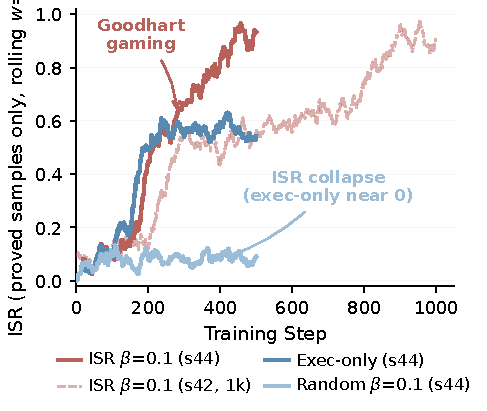
\includegraphics[width=0.82\columnwidth]{figures/fig5_training_isr_curves.pdf}
\caption{ISR$^*$ (proved samples only) training trajectories across reward conditions (rolling $w{=}20$). Exec-only collapses to $\text{ISR}{\approx}0$, confirming structural degeneration (\S\ref{sec:diagnostic}); the ${\sim}0.5$ plateau is an $n{=}2$ artifact. ISR $\beta{=}0.1$ seeds rise toward $\text{ISR}{\approx}1$ via TS gaming (Goodhart effect, \S\ref{sec:goodhart}); random remains low.}
\label{fig:training-isr-curves}
\end{figure}

Applied post-hoc, ISR reveals that rising prove rate conceals a compositional shift in proof structure: genuine reasoning gives way to hacking modes (conclusion embedding and tautological shortcuts), invisible to execution-based metrics (Figure~\ref{fig:training-isr-curves}; \S\ref{sec:diagnostic}).

Yet the same LOO structure that makes ISR diagnostic also creates a Goodhart vulnerability~\citep{manheim-goodhart-taxonomy, karwowski-goodhart-rl, gao-reward-overoptimization}: tautological formalizations ($P{\to}P$) satisfy the necessity criterion by construction, so when ISR is repurposed as a training reward, the model learns to game the diagnostic rather than the task.
Our results suggest that LOO-based structural proxies, and plausibly other component-necessity measures, face analogous exploitation risks in neurosymbolic settings.
In our Qwen3-4B experiments, the asymmetry persists across logic types (first-order logic [FOL], Prolog), reward doses, and random seeds, with dataset-dependent boundary conditions (FOLIO vs.\ ProofFOL; \S\ref{sec:crossdomain}), suggesting that structural proxies for formalization integrity are easier to observe than to optimize.

We contribute:
(\textbf{C1})~a systematic empirical analysis of structural degeneration in GRPO-trained neurosymbolic reasoning, using LOO ablation (STA/ISR) to catalogue eight hacking modes across six reward conditions (\S\S\ref{sec:sta}--\ref{sec:crossdomain});
(\textbf{C2})~empirical characterization of a seed-dependent Goodhart effect when ISR is repurposed as reward, with matched controls ruling out confounds (\S\ref{sec:goodhart});
(\textbf{C3})~cross-logic replication (FOL/Prolog) confirming that the Goodhart effect transfers across logic types, with exploratory cross-dataset evidence (FOLIO/ProofFOL; \S\ref{sec:crossdomain}).
